\section{Il bilancio di esercizio}

\subsection{Concetto di azienda(riepilogo)}

\subsubsection{In termini soggettivi}
Istituto economico dotato di autonomia e proiettato nel tempo, in cui si coordinano una molteplicità
di risorse per il raggiungimento dei fini stabiliti dal soggetto istituzionale.

\subsubsection{In termini oggettivi}
Insieme delle attività svolte dall'istituto nell'ambiente economico(azione econimica).

Sistema di azioni che si traducono in scambi con terzi finalizzati al raggiungimento di un fine economico.


\subsubsection{Caratteristiche dei beni e servizi oggettivi di scambio}

Utilità(soddisfacimento dei bisogni).

Scarsità(determina il valore economico di transazione e rilevazione)


\subsection{Rilevazione: principali funzioni}

Quantificare, misurare, rappresentare e interpretare i fatti aziendali.

\subsection{Metodi per la rilevazione}
\textbf{Contabili}: si servono del conto quale strumento principale delle rilevazioni.

\textbf{Non contabili}: altri strumenti.

\subsection{Il sistema contabile e le informazioni}
Le informazioni a cui il sistema contabile si può riferire possono riguradare:
\begin{itemize}
    \item situazioni di economicità globale(prende un grosso periodo in analisi)
    \item situazioni parziali(analisi parziale dell'attività)
    \item situazioni attinenti al rapporto tra l'azienda e le principali categorie di interlocutori esterni
\end{itemize}

\subsection{Contabilità}
Raccolta. misurazione, analisi, interpretazione, sintesi e comunicazione di informazioni
economiche.

\subsection{Funzioni della contabilità generale}
Processo organico e sistematico di rilevazione di fatti di gestione,
scambi con terzi(fornitori e o clienti) e utlizza lo strumento della contabilità
e il metodo della partita doppia per:
\begin{itemize}
    \item determinazione periodica del risultato e del capitale di funzionamento
    \item controllo delle posizioni finaziarie azindali
\end{itemize}

\subsection{Le operazioni aziendali}
Sono operazioni di gestione che vengono fatte di continuo e in modo simultaneo:


\begin{itemize}
    \item sono unità elementari dell'attività operatia
    \item diversa complessità
    \item possono essere interpretate all'interno del sistema e non solo in modo individuale
\end{itemize}

\subsection{Processo di produzione economica}
gestione finalizzata a:
\begin{itemize}
    \item condizione di gestione(organizzazione)
    \item fattori produttivi: generici e specifici(investimenti in macchinari, impianti, ecc)
\end{itemize}


Il capitale messo a disposizione dall'imprenditore o dai soci è il capitale di rischio.

Il capitale di credito sono i prestiti che terzi(si spera banche) fanno all'azienda(non mafia ecco KEKW).

Per il capitale di rischio non c'è un obbligo di restituzione, viene conferito o come messi monetari
o direttamente aggiungendo fattori produttivi e può essere conferito in momenti differenti.

Per la remunerazione si deve vedere come va l'azienda.

Il capitale di terzi(prestiti) deve essere rimborsato nella maniera stabilità insieme al terzo in questione.


\subsection{Il circuito della produzione}
I mezzi moentari vengono investiti in fattori produttivi, la fase di produziione si divide in aquisizione materiale,
processamento e vendita.

\textbf{La differenza fra ricavi e costi è il reddito}


I prestiti non rappresentano variazione della ricchezza aziendale, si segna soltanto 
la differenza fra denaro ricevuto e quello restituito(l'interesse) che è alla fine dei 
conti l'unico esborso dell'azienda.



\begin{figure}[H]
    \centering
    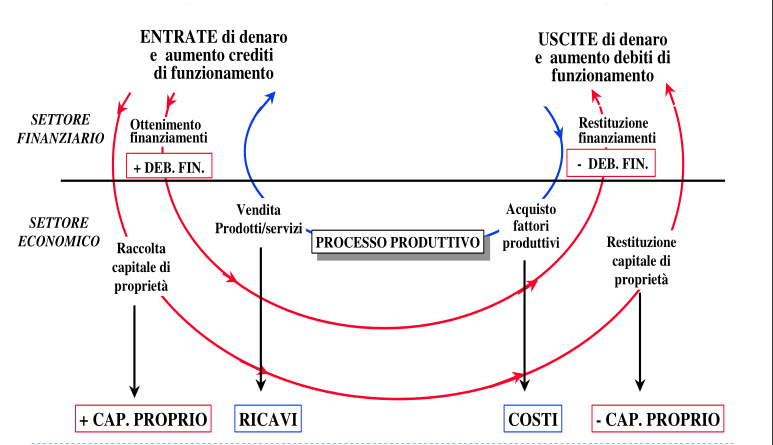
\includegraphics[width=0.7\linewidth]{2/img/Screenshot from 2022-07-05 15-52-30.png}
\end{figure}

\subsection{Classificazione variazioni di valore}
\subsubsection{Variazione finanziaria negativa}
\begin{itemize}
    \item diminuzione di denaro
    \item aumento debito funzionamento
    \item aumento debito finanziamento
    \item diminuzione credito funzionamento
    \item diminuzione credito finanziamento
\end{itemize}

\subsubsection{Variazione finanziaria positiva}
\begin{itemize}
    \item aumento di denaro
    \item aumento di crediti di funzionamento
    \item aumento di crediti fi finanziamento
    \item diminuzione debiti di funzionamento 
    \item diminuzione di debiti di finanziamento
\end{itemize}

\subsubsection{Variazione economica positiva}
\begin{itemize}
    \item ricavi
    \item rettifiche (diminuzione) dei costi
    \item aumento di capitale proprio
\end{itemize}

\subsubsection{Variazione economica negativa}
\begin{itemize}
    \item costi
    \item rettifiche(diminuzione) dei ricavi
    \item riduzione capitale prorpio
\end{itemize}

In sintesi:
\begin{itemize}
    \item Aspetto finanziario
        \begin{itemize}
            \item denaro
            \item credito e debito funzionamento
            \item credito e debito finanziamento
        \end{itemize}
    \item Aspetto economico
        \begin{itemize}
            \item costi
            \item ricavi
            \item capitale proprio
        \end{itemize}
\end{itemize}

\subsection{Aspetto finanziario ed economico dei fattori produttivi}
Divisione fra fattori produttivi che vengono usati una volta sola(fecondità semplice)
e altri fattori che vengono usati ripetutamente e perdono solo una porzione di valore al momento 
dell'utilizzo(fecondità ripetuta).

\subsubsection{Principio di correlazione}
Un fattore produttivo deve essere correlato alla realizzazione del prodotto che ha 
contribuito a creare.



\begin{figure}[H]
    \centering
    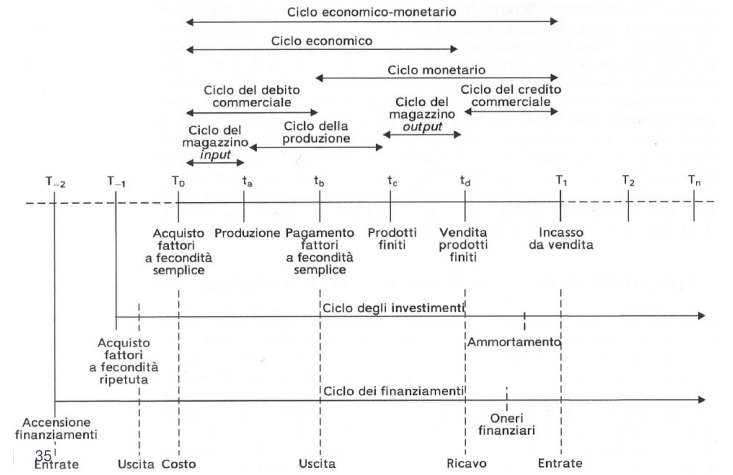
\includegraphics[width=0.7\linewidth]{2/img/Screenshot from 2022-07-05 16-11-59.png}
\end{figure}